\documentclass[12pt,a4paper,oneside]{report} 

%\documentclass[14pt,a5paper,oneside]{memoir}
%\setlrmarginsandblock{1cm}{1cm}{*}
%\setulmarginsandblock{2cm}{2cm}{*}
%\checkandfixthelayout

\usepackage[pdftex,
            pdfauthor={Jonáš Gruska},
            pdftitle={Streams & Currents},
            pdfsubject={Wireless Network Sonification and other works},
            pdfkeywords={sonification, wireless networks, soundart, installations},
            pdfproducer={LaTeX with hyperref},
            pdfcreator={pdflatex}]{hyperref}

\usepackage[utf8]{inputenc} 
\usepackage{xcolor}
\definecolor{red}{HTML}{AD1737}
\usepackage{hyperref}
\hypersetup{
colorlinks=true,
linkcolor=red,
citecolor=red,
urlcolor=red,
anchorcolor=red,
filecolor=red
}
\usepackage{apacite}
\usepackage{cmap} 
\usepackage{url}
\usepackage[T1]{fontenc} 
\usepackage[osf]{libertine} 
\usepackage{libertineotf}
\usepackage[scaled=0.90]{inconsolata}
\usepackage[parfill]{parskip} 
\usepackage{listings}
\usepackage{graphicx}
\usepackage{float}
\usepackage{setspace}
\usepackage{anyfontsize}


\onehalfspacing
\usepackage{tikz}
\usetikzlibrary{shapes,arrows,fit,backgrounds}


\title{
{\fontsize{43}{30}\selectfont \color{red}\sc{Streams~\&~Currents}}\\
{\fontsize{15}{15}\selectfont \emph{Wireless Network Sonification and other works}} 
}

\author{Jonáš Gruska\\
Bachelor's Thesis\\
Institute of Sonology} 

\date{}

\begin{document}

\frenchspacing
\raggedbottom
\doublehyphendemerits=10000       % No consecutive line hyphens.
\brokenpenalty=10000              % No broken words across columns/pages.
\widowpenalty=9999                % Almost no widows at bottom of page.
\clubpenalty=9999                 % Almost no orphans at top of page.
\interfootnotelinepenalty=9999

\maketitle

\begin{abstract}
First and main topic of this thesis is a concept of sonification and its various sub-methods. It deals with few examples of the significant works from the area and it is presenting a specific division of the sonification into a scientific and an artistic world.
Second topic is my own artistic work, which partly overlaps with sonification, but also reaches towards site-specific audio-visual installations, compositions based on a auditory illusions and the minimalistic gallery performances. 
\end{abstract}
\clearpage
\setcounter{page}{3}


\chapter*{Acknowledgements}
I would like to thank my parents for supporting me during my studies. I would never be able to learn what I love without them. And of course, I would like to thank my mentor Paul Berg for his patience with my chaotic behavior and the whole Institute of Sonology for helping me to become who I want to be. Lastly, I would like to thank Janka Kobolková, Marko Uzunovski, Xavier De \mbox{Wannemaeker}, Maya Verlaak, Daniel Tóth, Peter Sych, Marek Chołoniewski and all my other friends in supporting me in my work, inspiring and pushing me forward. My special thanks go to Marek Slobodník, Norman Teale and Agnes Szelang for helping me with my language.

\hypersetup{linkcolor=black} 
\setcounter{tocdepth}{1}
\tableofcontents
\hypersetup{linkcolor=red}

%%%%%%%%%%%%%%%%%%%%%%%%%%%%%%%%%%%%%%%%%%%%%
%%%%%%%%%%%%%%%%%%%%%%%%%%%%%%%%%%%%%%%%%%%%%

\chapter{Introduction}

My work has never focused on single topic, yet there are connecting traits in all of it. \emph{Streams and Currents}, as in streams of data versus electric currents can be one of those traits. My passion for the pure informational flow surrounding us in various forms is more than hinted in many of the topics I describe.

Sonification has grabbed my interest since my first experiments with programming computer music. By the time of my first contact with the method, I was amazed by the possibilities presented by software such as Pure Data, where one could easily turn data-flows into their sonic representations. Using external streams as sources of inspiration seemed very rewarding, in terms of conceptual and practical realization. Not surprisingly, the method stuck with me for some time.

This is the reason why I have chosen topics of sonification as a key element to my thesis---it serves as one of the main inspirations to many of my works in various degrees. In the next chapters, I will try to describe the context of my work with a few significant examples and comparisons from the art world and the world of science, to give a better idea of where my ideas started. I will also attempt to distinguish two separate traits in approaches towards sonification, relevant for sonological context, and I will try to give an overview of devices which allow us to sonificate \textit{in situ}, the ones with a scientific goal and those with purely aesthetic use.

After the topic of sonification, I will describe several of the most important projects I have worked on during my years at Intitute of Sonology (2009--2013), which should help to define my artistic approach in examples. This approach might not appear coherent at first, but one might notice that my work always shares specific qualities. A passion for technology, which is often present but not visible, a love for sound as the pure physical vibration of the air, and an effort to turn the invisible into the audible.

This specific style of work is not something I have been developing consciously, one could say it came more from within. I was drawn towards technology since I was a child, spending endless hours in front of the flickering screens and lately in a cloud of soldering fumes. But technology by itself does not satisfy me, and I am trying to see beyond engineering, through the streams of electrons. Because my intrinsic power is sound. But I need bits and volts to reach it.

%%%%%%%%%%%%%%%%%%%%%%%%%%%%%%%%%%%%%%%%%%%%%
%%%%%%%%%%%%%%%%%%%%%%%%%%%%%%%%%%%%%%%%%%%%%

\chapter{Sonification and audification experiments}

\section{Thoughts on current state of sonification}

The topic of sonification is intriguing for few reasons. Firstly, it benefits from the interest of various groups of people---scientists: biologists, mathematicians; creatives: musicians, sound artists; and the general public. Another is a belief, that this topic still has a lot of unrevealed potential. I will try to discuss the clash between the scientific and artistic approach, various significant projects or artworks, as well as fields of opportunity blossoming from this duality.

The main understanding of the term \emph{sonification} is the \emph{``use of non-speech audio to convey information''}, or more precisely, it is the \emph{``transformation of data relations into perceived relations in an acoustic signal for the purposes of facilitating communication or interpretation''}~\cite[p.~1]{Fitch}. These are definitions from probably the most relevant institution in sonificication---the International Community for Auditory Display~\cite{icad}, which has been organizing conferences and publishing books on the topic since 1992. Nicolas Collins puts it less formally, as a method for one to provide \emph{``aural alternatives to pie charts, line graphs and spreadsheets''}~\cite[p.~7]{Collins2006}. All these quotations define it as an analytical, representative point of view, and the reasoning behind the use of sonification in this sense is repositioning of the information from the traditional semantic, visual or statistic level to the sonic level giving ground to non-traditional data analysis via sound or music. Interestingly, ICAD's first definition mentioning conveying \emph{information} rather than data can also give an understanding of the fact that sonification is not only about data patterns; and whether we try to sonify weather forecast, biological systems or our emotions is not important---they are all qualified.

I believe the analytical approach towards sonification is rather clear and well defined. Books such as the Sonification Handbook~\cite{Hermann2011} prove that ICAD and its fellow researchers have done exquisite work in examining the topic from various points, resulting in apparatuses which artists can build upon. Although the arts and sciences have many things in common, aesthetic approaches toward sonification projects are in my opinion quite different.

That is why I would like to propose a division in this definition. There is one part of sonification world, described above---that is, an analytical, `auditory display' world. My proposition adds \emph{an artistic world}, where the main goal of the process is not to make certain data accessible for aural analysis, but rather to use those data as a essence of specific aesthetics. That means, one is no longer looking for a scientific tool, but a sonic instrument, a source of inspiration and compositional data. It might also be described as a matter of aim behind the use of sonification methods: whether works are aimed to inform a listener or provide him an auditory display of some data, or whether they are used for their characteristic aesthetics.

Use of streams of data for compositional and sound generating purposes is very familiar to electro-acoustic composers, artists and performers. Sonification in the artistic view is pushing the idea a little farther---instead of algorithms, \emph{real world} data are used, although reaching their exact, understandable representation becomes additional or even insignificant, rather than essential. It might be, that there is a deeper meaning behind the selection of the data stream (when artist sees the action as political act), so it is important that the point I am describing is more theoretical---real works are more often combining certain degree of aesthetics with conveying information through sound.

To give some real world examples, I would like to point out few significant works which use sonification as its main concept or method, and while doing so, I will try to exercise my proposal for the new sonification definition division.

One of the most classic examples of sonification is the \emph{Geiger} (or \emph{Geiger-Müller}) \emph{counter} particle detector which measures ionizing radiation. This tool is known for its direct connection between environmental value (in this case, radiation) and sound, and is one of the most known sonification tools. Technically, the method of auditory display of the information is the use of pulses---representations of electrical charges (and consequential discharges) of the inert gas in the {Geiger}-{Müller} tube caused by particles or photons of the radiation. Higher amount of electrical discharges (which translated into a higher number of audio pulses coming from the speakers) signals a greater density of particles of the radiation, thus higher radiation in the environment~\cite{Knoll2010}. A Geiger counter is clearly an \emph{analytical} sonification tool, with its main purpose being the representation of certain information, rather than using the information as an artistic basis.

I have chosen the Geiger counter for another reason, apart from it simply being the ideal representation of scientific and analytic attitude towards sonification. It is also a standalone and portable instrument. This opens up a possibility for its artistic use, even though its design is serving purely for research purposes. As I suggest later on in subsection discussing my wireless sonification project, I find interest in portable sonification tools for various environmental experiments. These tools can be used as an immediate instruments, serving artists with unconventional musical experience of the data \emph{in situ}.  

Geiger counter can be also viewed as representation of a sub-method of sonification, \emph{audification}. To quote the Sonification Handbook,  \emph{``audification is a technique of making sense of data by interpreting any kind of one-dimensional signal (or of a two-dimensional signal-like data set) as amplitude over time and playing it back on a loudspeaker for the purpose of listening''}~\cite[p.~301]{audif}.

Audification is sonification simplified to the most basic level. The majority of the common real-time sonifications are then audifications as well, e.g.\ listening to the whale songs or bat echolocation, where the only transformations which happen on the data are changes of the playback speed.

One of the most interesting sonification works is the work of Christina Kubisch~\cite{ChKubisch2012}. I have chosen her as an icon of electromagnetic induction, even though there is a wider spectrum of artists using the same tools. She generally appears as the icon of the method, so it will not be different in this thesis. Kubisch is a German sound artist born in 1948. She studied classical instruments such as flute and piano, but later turned to studying electronics at the Technical Institute of Milan. Since then she has created various sound installations, usually combining electronics and delicate sounds. In a work I would like to mention---Electrical Walks, Kubisch is focusing on audification of electromagnetic fields with the use of induction coils, headphone amplifiers and headphones. This works as a nice example of artistic audification, where the purpose seems to be to find interesting sounds within the world of electromagnetic fields rather than scientific analysis. 

Induction coils act as antennas and natural amplifiers, which when in the right setting, can provide excellent tools for electromagnetic sensing. Alternating current (AC) oscillations of the electromagnetic field are inducted on the coil, thusly creating AC signal. This AC signal is then amplified and can be directly treated with any audio devices as sound. It is an oscillation, similar to the signal produced by oscillators.

I have designed a simple pocket amplifier for these purposes called \textbf{Eletrosluch} (see fig.~\ref{fig:elektrosluch}). This device provides 100x gain for the coils and it is powerful enough to drive headphones. Its main benefit is size and portability, ideal for an electromagnetic sonic explorations. The version 1.0 used a tape head which I have extracted from an old tape player as the induction coil. The amplifying circuit was based around LM386 amplifier, which I have replaced in v1.1 with a low-noise operational amplifier TL071. Tape heads have been replaced with \emph{pick-up coils}, which were, in the previous century, used for noise-less recordings of telephone calls by means of attaching the with suction cups to telephone headsets. 

\begin{figure}  
  \centering
    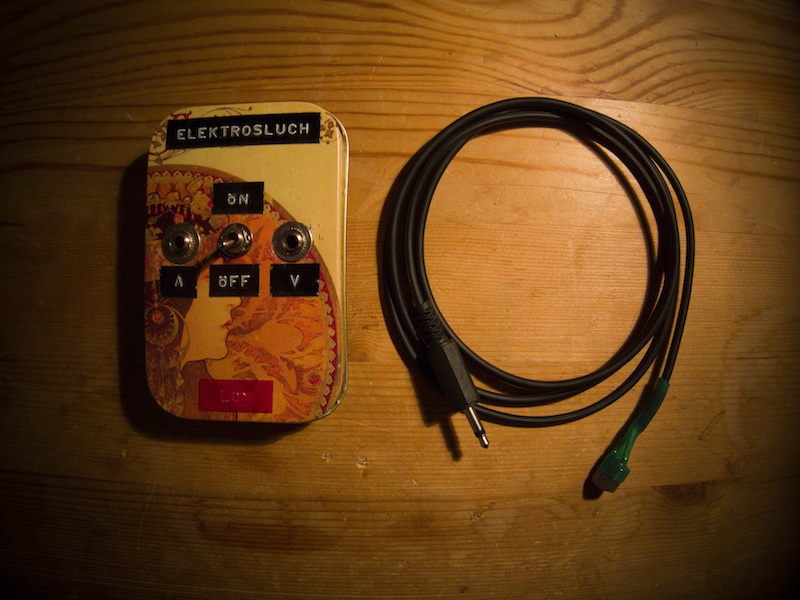
\includegraphics[width=0.9\textwidth]{img/elektrosluch}
	\caption{Elektrosluch 1.0}
	\label{fig:elektrosluch}
\end{figure}

Probably closest to my network sonificiation work is the one by Michael Chinen  and Shintaro Miyazaki's Institute for Algorhytmics. 

Michael Takezo Chinen is an American programer. He studied computer science and composition at University of Washington, Tokyo Denki University and Dartmouth College with Richard Karpen, Charles Dodge and Naotoshi Osaka. He was part of the developers of the popular open source audio editing software Audacity. His artistic focus resides in software sonification, in the sense of a method as in sense of a target. His proof to this claim are his works \textbf{lstn} and \textbf{FuckingWebBrowser}, which I will now try to examine in greater detail.~\cite{mchinen}

Both \emph{lstn} and \emph{FuckingWebBrowser} are based around sonification of computer based streams and data. To be more precise, lstn is \emph{``a program that sonifies real-time debugging data of other programs''} and FuckingWebBrowser is \emph{``simple mac web browser with memory sonification based on WebKit''}~\cite{Chinen2010, Chinen2010a}.

These works are quite similar to my work Sonodump (see~\ref{sec:wifi}). For example, as well as Chinen in FuckingWebBrowser, I also deal with browsing of the internet as with the initial trigger and data stream for the sound generation. One might find it as analogous action to e\.g.\, bowing of a violin. Address bar becomes a bow and stream of data (conscious decisions about URLs to type in the address bar) is the angle and pressure of the bow on the strings. 

Chinen makes an excellent point for an artistic stand towards sonification. The aim towards translating real information to the listener is missing (maybe only to a very experienced one); use of sonification plays a different, artistic, role, rather than the one of auditory display. It is about using a pure source of data for sound generation, not a source of information meant to be mediated towards an audience.

His work is representative and direct, yet its main point is not to convey information. Auditory display becomes `useless' from scientific or research point of view and becomes interesting as an artwork for its specific aesthetics.

Chinen's work has been strongly connected to the Institute for Algorhytmics, led by Shintaro Miyazaki. He is a post-doctoral researcher at Humboldt University in Berlin dealing with \emph{``epistemology, archeology, history and theory of everyday technologies, which store, transmit and process informations and their dynamic relation to sound, rhythms and other sorts of time-varying signals''}~\cite{Miyazaki2012}. From his projects, I want to point out his collaboration with Martin Howse~\cite{howse} called \textbf{Detektors}.

Detektors is \emph{``an open, collaborative project which uses sonic strategies and DIY-devices to make audible the hidden infoscapes of our time. The present website will show data, recordings and cartographies of different spectral ecologies and trans-sonic machinic agencements''}~\cite{detektors}. The website of the project contains many sound recordings of the electromagnetic fields (audifications) from radio-frequency range as well as cartographic information about such sources. It is a study of the electromagnetic pollution, sonic behavior of digital devices in the context of a geolocational sound recordings.

\begin{figure}  
  \centering
    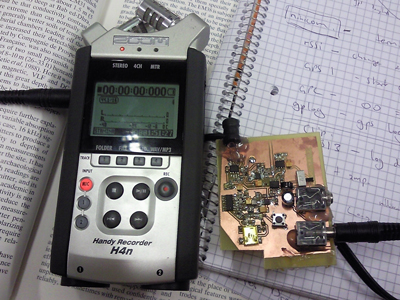
\includegraphics[width=0.9\textwidth]{img/detektor}
	\caption{Detektors \emph{Detektor} device}
	\label{fig:detektor}
\end{figure}

A specially designed device is used for the `detection', as seen on figure~\ref{fig:detektor}. The core of the hardware is a logarithmic detector chip AD8313 produced by Analog Devices. This chip takes AC signals from up to 2.5 GHz  (upper border of the most used wireless network range is 2.4 Ghz~\cite{802} and demodulates them into audible sphere. This is somehow similar to the work of Kubisch, but there is a difference in the frequency spectrum target. The method using induction coils leaves us only with electromagnetic AC signal within our hearing range and within the limitations of the amplifying system, but the method of using demodulator allows us to listen to high frequency communication, such as bluetooth and wireless radio. Interestingly, Detektors and Kubisch's work both share emphasis on placing of their sonic discoveries within cartographic space.

These works have proven to be very effective in their directivity and immediacy. One can simply turn on the device and listen to `invisible' streams of data, constantly present and surrounding, yet unnoticed by our senses. 

My Wireless Network Sonification work is strongly related to that concept. My passion for revealing omnipresent data streams, penetrating our tissues on a daily basis is possibly very similar to what has driven Kubisch or Miyazaki to build their own sonification systems.  

But before I jump to describing my works, I want to mention one more example of sonification project: a project of Gil Weinberg called \emph{BrainWaves}. It is based on interactive auditory research of electrical stimuli applied to \emph{in vitro} neuron cultures. I picked this work for the inherent collision of scientific and artistic approach.

To briefly describe the project, \emph{BrainWaves} is \emph{``sonification installation that allows a group of players to interact with an auditory display of neural activity. The system is designed to represent electrical spike propagation in a neuron culture through sound propagation in space. Participants can simulate neural spikes by using a set of specially designed controllers, experimenting and sonically investigating the electrical activity of the brain''}~\cite[p.~9]{Weinberg2006}. The particular part which caught my interest is the desire to experiment with the subject of sonification interactively. The classic idea of stream of data is missing---instead of discrete information there is a system, which needs to be sonified. As a comparison, one can imagine hitting an oil barrel in a goal of exploring its acoustic properties---physical model, where system becomes the subject.

Since the main subject of the auditory display is propagation pattern simulation, the authors have decided to use spatialization as a key element of representation. As they argue against visual display, \emph{``sonification can be more effective than visualization in such a spatial application because the human auditory system is able to perceive synchronous spatial stimuli from every point within a space, while visual perception is limited to physical range of sight''}~\cite[p.~9]{Weinberg2006}. For the purpose, 8 speakers in space are used to provide sufficient clues for the exact propagation pattern.

For the interactive standpoint, custom made drum trigger instruments were created using piezo elements to represent electrical spikes in the system. Performers are asked to hit these in specific way---after first propagation ends, performer placed closest to its ending is bound to start another one, by hitting his own instrument. At this point one could see an interesting connection between \emph{sonification} and \emph{gamification} as a very close methods of bringing data streams and system under closer, possibly more understandable, examination.

As the authors conclude, the method of using almost only spatialization for auditory display purposes was not completely successful, since they noticed that part of the performers was using visual representation of the process (provided during event) to orient in the process rather than simply \emph{listening} to the positioning. 

From the analysis stand point, I see this work as bordering between the scientific and artistic approach. The effort to analyze real scientific system combined with use of almost musical methods and instruments seems as an interesting way of reaching sonologicaly relevant results. It appears that authors have not seen scientific results as a pure purpose of the work. Using (musical) instruments, focus on aesthetics of the sound themselves both suggest this was not classical scientific approach.

Hopefully, at this point I have presented sufficient amount of various works which allow me to prove my point in making distinction in methods or approaches in sonification. I personally believe, that it is important to recognize artistic sonification as specific subject, since I have not found this disambiguation to be done sufficiently.

%%%%%%%%%%%%%%%%%%%%%%%%%%%%%%%%%%%%%%%%%%%%%
\clearpage
\section{Wireless Network Sonification}
\label{sec:wifi}

As a part of my own experimentation with untraditional sources for musical or generally sonic data I decided to extend my line of work on the layer of wireless networks. The project I would like to describe in this chapter deals with wireless network sonification as a main artistic source for sonic performance and installation. In basic terms, it catches data streams `from the air' and transforms them directly into sound using a set of tools and methods. This work has been presented as a performance and an installation. In case of performance, I have used the live coding technique to change the aspects of the sonification. This was done via purposeful tampering of the networks by creating artificial data streams as well as by modifying the parameters of sonification.

\subsection{Work process and technical details}

To describe the process in higher detail, I would like to define some basic terms of the technical side of the project first, and then continue by describing my point of view on an even more important artistic side.

I will start with packets and packet analyzers, since they are key elements of my wireless network sonification efforts. Packets, and in this case \emph{network packets} are units of formatted data. It is basically a standard of packing a predefined amount of information into a understandable format, easily and efficiently transmittable over networks. \emph{Packet analyzers} or \emph{sniffers} are tools for silent interception of network traffic. In technical terms, it is software (or hardware) which passively receives all data link layer frames passing through the device’s network adapter, not just those directed towards recipient. They are generally used by hackers, while also having legitimate use by system and network administrators or security experts. Sniffing is possible due to the physical characteristic of network. Either with LAN (Local Area Network) or unencrypted WLAN (Wireless LAN), all data passing through the system are accessible to everyone. It is then a job of WLAN or LAN adapters (network cards) on the site of client to separate its part of the data using filtering based on the MAC (Media Access Control) address. A MAC address is an unique identifier of every computer's network adapter. Except simple network MAC filtering, it can be, e.g.\, also used for assigning IP address by ARP (Address Resolution Protocol) and DHCP (Dynamic Host Configuration Protocol).

By enabling the functionality of network device called \emph{promiscuous mode}, one is able to avoid this filtering and obtain all present network packets. This is possible  for both wired and wireless adapters, thus for both wired and wireless networks. Of course, there are certain limits to this. For example when a \emph{network switch} is placed in the network, it is not possible to receive everything. Network switch, different from \emph{repeater} or \emph{hub} (device only physically `multiplying' the cable), is a more advanced device and acts as a MAC filter by itself, therefore working as a network filter by itself.~\cite{Pallavi2012}

A classic example of a sniffer is \textbf{tcpdump}. Tcpdump was developed at the University of California in 1987 by Van Jacobson, Craig Leres and Steven McCanne and its main use is traffic analysis. The Unix Manual entry describes it as ``dump traffic on a network''~\cite{tcpdump}, but that is very reducing. Over the years since its first release it has become a rather complex and powerful tool. One of the features of tcpdump is that it can work easily with both LAN or WLAN packets (and actually many other obscure network protocols) and therefore provides us with various data sources for our artistic purposes. Because of its enormous functionality on one hand and lightweight operation on other, it has become my favorite tool for wireless network sonification and will be discussed more, later on in the text.

In the beginning of my research I was considering few options, ways, and processes. I was motivated to learn C programming related to audio, so that became my first choice. It has started by writing my own sniffer, based on library developed by same developers as the ones of tcpdump. This library is called \textbf{libpcap} (PCAP stands for Packet CAPture) and serves for implementation of tcpdump functionality to one's software. Obviously, this was not very easy task to do, especially for an unexperienced C programmer such as myself. After I finally managed to sniff data using my software, the next step was to use \textbf{PortAudio} library to implement the audio part of the project.

Finally I partly succeeded, by writing \emph{Sonodump}. Sonodump worked closely to what I wanted---it \emph{sniffed} the network data and reflected current traffic via sound. The conversion was done through treating data harvested from the network as audio data---a simple WAV file. The user had only two options to select from: which interface should be used (wireless or wired) and what sample rate is expected. Use of the term sample rate is a bit inaccurate, because there is no correct, real sample rate of the stream---it is not an audio stream. We can just guess or purposefully select some value to affect the way the sonification behaves. Lower sample rates resulted in a rather low-frequency based sonic content and higher settings create more higher frequencies. This occurs simply because of the speed the network data are read. It can be described as an obscure case of wavetable synthesis with tables generated by the network stream.

Sonodump already gave some interesting results, yet it was not very efficient. My programming skills were not just on the right level to optimize the code properly. Therefore I needed to look for other options. In autumn 2011 I was asked by the organizer of the AudioArt festival in Krakow, Marek Chołoniewski to present my sonification work on his festival. I happily agreed and immediately thought of the wireless sonification project. But Sonodump was not enough in this case---I needed something more flexible, powerful and in the end, more interesting.

One of the questions was whether to treat the sonification process in a more traditional way, lacking interaction with the stream which is being sonified. I felt inner conflict between keeping certain level of purity and working on the most successful and pleasant aesthetic experience. In the end, the idea of live interaction with the stream of data won, with argument planning for achieving non-traditional way of control over the resulting sound. With image of this wild, partly unpredictable instrument I started to research other, new technical solutions.

As mentioned before, Sonodump was not optimal and had a few problems (in programmers lingo---bugs), but after some time, I discovered other very useful set of commands present on Linux systems.

The main motivation for working with Linux / UNIX was the availability of all the tools which I required (sniffer, network tamperer, raw data stream player) and system shell, terminal. This shell allowed me to do scripting (basically programming with advanced tools) and very importantly for this project, \emph{pipelining} and \emph{redirecting}---interconnecting processes and files. For example, output of one a process can be streamed in real time to an another without user caring about any `middle-man' text file or thinking about memory allocation. This comes in particularly handy, when one wants to \emph{sonify} something. 

Good example is redirecting of a non-audio file to the sound card. What this represents is treating the file as a stream of data consequently feeded to the sound card as it would be audio data---coming for example from a mp3 player. On some Linux distributions (Linux comes in various flavors) it is enough to write this command to the terminal:
\begin{quotation}
	\texttt{\textbf{\$} cat SONIFY\_ME.txt > /dev/dsp} 
\end{quotation}

Command \texttt{cat} reads the file \texttt{SONIFY\_ME.txt}---which is a regular text file; and by using the symbol \texttt{>}, bash takes care of writing it to \texttt{/dev/dsp}---which is a virtual port for the sound card. Writing to this port opens a stream on the sound card and plays the given data as audio.

This is very primitive and direct method of sonifiying any data and sometimes results in quite surprising compositions. It is not an easy task to determine whether this primitive mode of sonification can be called composing and who actually is a composer in the system. Is it me, the person which conceptually combines data stream and their sonic interpretation or is it the program which actually decides on the translation of the data to sounds? I believe that the result of sonification of a non-audio data file can be seen as a composition, but I am not completely sure who is the composer in that situation. I am generally inclined to the idea, that the program, data file and my concept are composing in \emph{symbiosis} of the Machine, Data and the Human.

I was particularly charmed by the sound of an archive containing source codes of tcpdump itself. The song (or a file---in this sense it is almost synonymous) offers range of gestures which are composed in a unexpectedly pleasing way. There are even appearances of few rhythmic patterns and primitive melodies. To give you a clear image, I have linked a recording of this composition in~\autoref{appendix:a}.

Basic process of reading network data and converting them directly to sound is not much harder. The \texttt{cat} command is now replaced with \texttt(tcpdump), which is a tool mentioned before---traffic analyzer, \emph{sniffer}.
\begin{quotation}
	\texttt{\textbf{\$} tcpdump -i wlan0 -A > /dev/dsp} 
\end{quotation}

Tcpdump opens a packet capture process at a device \texttt{wlan0} (wireless module). Option \texttt{-A} represents conversion of the captured data to ASCII symbols, allowing us to always read them in the terminal as text. These are then again, streamed into \texttt{/dev/dsp} which serves as the sonifying module. This already gives us some amount of sonification of the network with just single line of code. 

Next step was, to think about what other ways are there to experiment with. One of the options was change of the sample rate of the /dev/dsp (sound card) on-the-fly and thus change of the resulting sound as with the Sonodump. After some research on the topic it seemed as rather complicated and bulky approach, so I had to think of some other method. That was when I discovered \textbf{aplay}, part of ALSA. ALSA is amongst OSS and Jack one of sound systems used for audio on Linux. The most important function of aplay for me was the possibility to read data from pipeline (i.e.\ from other process) and to modify a few parameters of the reading. Great addition was fact, that it is easy to have almost unlimited amount of aplays playing at the same time, even from one source. ALSA is handling the mixing of the streams to the sound card.

Interaction (or as some people call it---tampering) with data stream was, as I mentioned earlier, not an easy decision. There was part of me trying to preserve the original streams in their pure form, but in the end, I have decided to work with streams as with a live instrument. Of course, the control is not as direct as hitting the drum. My \emph{stick}, which I use to hit the system, is hidden in the terminal. 

\begin{figure}  
  \centering
    \tikzstyle{block} = [
		rectangle, 
		draw, 
	    text width=6em, 
		text centered, 
		minimum height=2.8em, node distance=4.5cm, scale=0.8, 
		%top color=white, 
		%bottom color=black!10, 
		rounded corners=2pt]
	\tikzstyle{line} = [draw, -triangle 90, scale=1.2]
	
	\begin{tikzpicture}[node distance = 2cm, auto]
	    % Place nodes
		\node [block] (nds) {Network data stream};
		\node [block, above of=nds, node distance=3cm] (rni) {Router, other network users};
		\node [block, right of=nds, node distance=4cm] (sniffer) {\textbf{tcpdump} \\Packet sniffer};
		\node [block, right of=sniffer, node distance=4cm] (aplay) {\textbf{aplay} \\ Actual sonification};
		\node [block, below of=sniffer] (me) {\textbf{Me} \\ (Performer)};
		\node [block, right of=aplay, node distance=4cm] (aout) {Audio output};

		% Draw edges
		\path [line] (rni) -- (nds);
		\path [line] (nds) -- (sniffer);
		\path [line] (sniffer) -- (aplay);
		\path [line] (aplay) -- (aout);
		\path [line, rounded corners=5pt] (me) -| node [near end, above, scale=.8, rotate=90] {Arbitrary data} (nds);
		\path [line, rounded corners=5pt] (me) -| node [near end, below, scale=.8, rotate=90] {\begin{tabular}{l}
		Sonification\\ parameters 
		\end{tabular}} (aplay);

		\begin{scope}[on background layer]
		    \node[fill=lightgray!50,inner sep = 3mm,fit=(aplay)(sniffer),label=above:Computer] {}; 
		\end{scope}

	\end{tikzpicture}
	\caption{Data flow of Sonodump performance}
	\label{fig:wifisonifi}
\end{figure}

From technical view, I was mainly generating arbitrary traffic using a set of tools created by hackers (penetration testers in everyday job) dedicated to stress testing of networks. Creating such artificial loads is useful for a few reasons: one being recording a reaction of routers to such massive amounts of data and the other one (a bit more evil one) is a bit more complex. When a router crashes because of an overload, all users on the network must reconnect. And reconnecting means resending passwords as well, so it creates ideal situation for sniffing of the sensitive data.

My use was obviously less malicious, I was experimenting with the behaviors of the sonic output under various kinds of attacks. To get a good overview over the whole process, see~\ref{fig:wifisonifi}. I have sketched the basic concepts of the different aspects of the system, which should help you to understand flow of information and the consequent transformation to audible domain.

At this point I have had prepared a sufficient toolkit for my upcoming performance and installation, therefore I started to focus on the artistic aspects, nuances of the work.

\subsection{Performance and Installation}
I have performed only once with this setup. As mentioned, it was on AudioArt festival in Kraków and it has been successful, for few various reasons. My initial approach was to try to create some kind of static object in space, which would then perform \emph{for me}, as in---instead of me. I would be sitting away from the device with laptop in my lap and I would control the process from there, over network. This has been the idea until around 4 days before the performance, when after talking with my friend I have decided to twist my plan in quite radical fashion and do a live welding of my instalation during the performance.

To elaborate a bit more, I have always been intrigued by welding and the atmosphere it establishes. Extremely, harmfully bright lights, bursts of current through metals, high voltage buzz. Sonically, sound world of welding machine was actually quite matching to sound world of my wireless sonification software. But that was not the only reason behind the use of such different instrument. From the beginning, I aimed to build specific kind of a sculpture, and 4 days before the performance, it still was not ready. The plan for the object was to create a pyramid from metallic rods, which would serve as representation of antenna, \textit{prism for streams}. Therfore, it clicked, and I decided to built one, during the performance, with the use of the welding machine.

\begin{figure}  
  \centering
    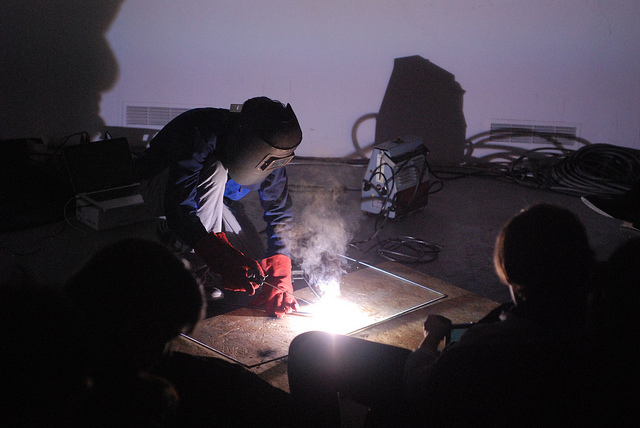
\includegraphics[width=0.9\textwidth]{img/zvarac}
	\caption{Sonodump performance}
	\label{fig:zvarac}
\end{figure}

I was not an experienced welder at all, I have welded only two times in my life before the performance. This was supposed to scare me, but it only drove me further---I acquired all the necessary protection, such as special welding protection helmet and gloves, and started to experiment. It was the day before the performance. Interesting note might be, that the venue had to change their circuit breakers in the power grid for higher current draws, all because of my performance.

During the performance, welding did a terrific job on creating two things. First being the already mentioned atmosphere---smell of hot metals, crackling and sizzling of the electric current were simply wonderful and spectacular. When I talked to the people from the audience after the performance, many have mentioned the connection to the welding happening `on the streets'. Everyone has few experiences with welders and the bright light of the process, which actually connects to the second aspect I managed to create. 

That was the fact, that since I used dangerous amounts of light (welding light can burn parts of the lenses), people have closed their eyes. While performing, I was of course focused on the performance itself, but when I saw video from the event, I noticed that most of the audience has either closed eyes or their heads are turned to the ground. Many faces just reflected pure focus on the sound. This was of course an amazing effect, which I actually did not expect to happen in first place. Since I was basically forcing people to look away, they really did and listened.

The installation was continuing in similar manner as a performance. By using \textbf{bash}, shell scripting language, I was able to create various simulations of myself. I programmed a simple robot, which was starting attacks on the local network, the same way as I would. This allowed me to create installation which was interesting enough and could have been presented in place for longer period of time without my attention.

Unfortunately, I have ran into problems with the installation during weekend, since gallery owners were turning their routers off for that period (since no one was working in the offices). Therefore, wireless sonification did not work for a few hours, since there was no network to be sonified. Fortunately I managed to provide my own router and setup my own network in place shortly.

\subsection{Future}
I am still intrigued by the network sonification, and I am at the moment working on a new projects these days. One is recreation of Sonodump called \textit{Hlysnan}, designed to be more user friendly application for Mac OS X and Linux. The aim of this application is to give visual feedback to people (displaying of the raw data streams), as well as live control of the sniffing and sonificating parameters via graphical user interface of the software. The project is still in its alpha stage. For the core of the software, I have migrated to C++ with use of OpenFrameworks framework for interface development.

The second project is not realized yet, but connects my idea of wireless sonification to handheld devices (as mentioned earlier). With the use of affordable computers such as the Raspberry Pi, I want to create a pocket device which would allow one to simply walk around and \emph{listen to networks} in a mobile way. So far I have it working as easily deployable small box for quick sonifications, but it would be nice to have physical interface for the interaction with the sonification and the sniffing process.

\begin{figure}  
  \centering
    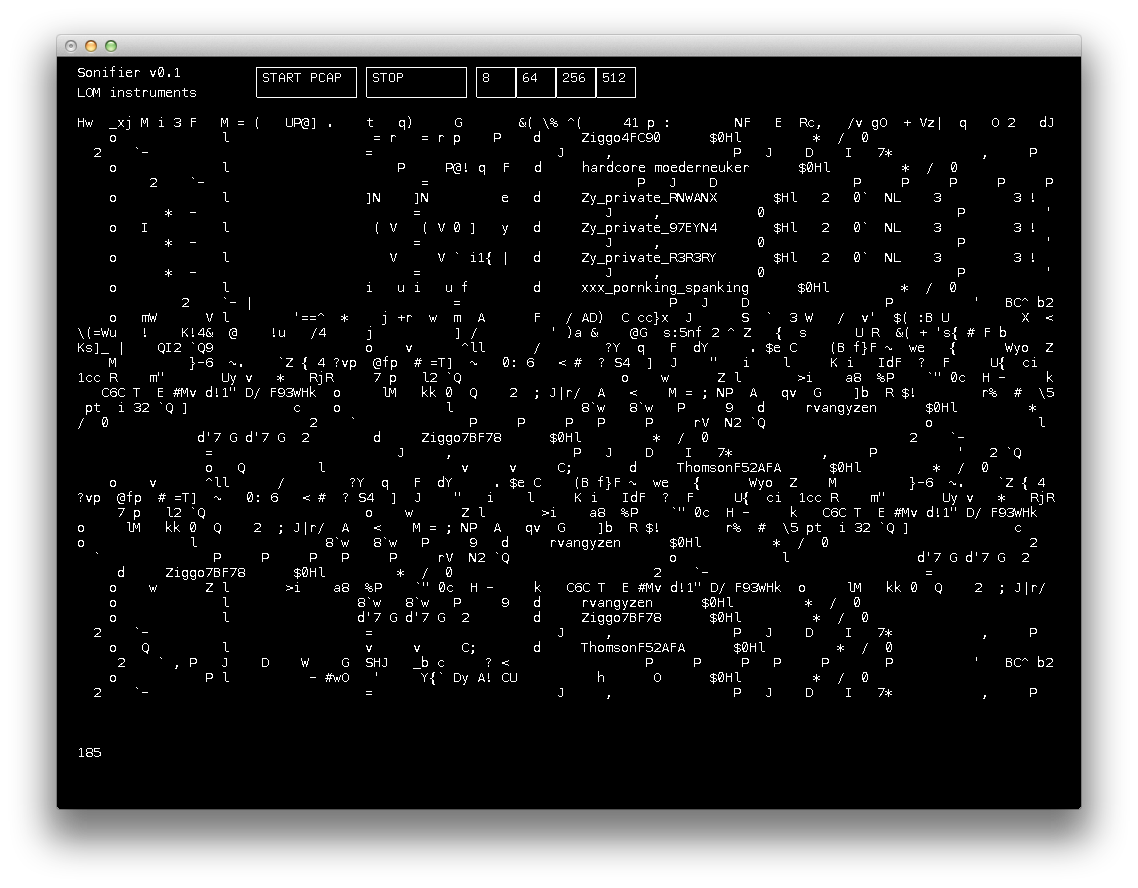
\includegraphics[width=0.95\textwidth]{img/hlysnan}%
	\caption{Hlysnan v0.1---reinventing the sonodump. In this screenshot we can see the minimalistic user interface as well as a portion of the sniffed wireless data.}
	\label{fig:hlysnan}
\end{figure}

%%%%%%%%%%%%%%%%%%%%%%%%%%%%%%%%%%%%%%%%%%%%%

\clearpage
\section{City Attributes Sonification}

\emph{City Attributes Sonification} is a project that I have worked on in 2011 in the Czech Republic. At the time, I was invited to lead a workshop on topics dealing with sound, city, and architecture. The event was a part of the bigger festival dedicated to the city of Brno.

The festival organizers happily accepted my proposal for the exact topic---the sonification of the city. I was very curious to see what people would come up with and it actually turned out very well!

The workshop lasted for 4 days. In the beginning I introduced the basic concepts of sonification and audification, presented a few significant (yet varying) works in the field, and then commenced with the brainstorming. Afterwards, we continued the brainstorming sessions regarding specific projects and worked on the technical realizations.

The workshop resulted in a few interesting ideas. One of the most inspiring works was the piece by Lucie Vítková. Lucie went on to study at the Royal Conservatory for a year after the workshop. Her idea was to do a direct/live sonic interpretation of the street. In the beginning, we split the street into sections and each participant was responsible for the sonification of his/her part. Each of us had different instruments and different sets of rules. The sonifications worked via visual cues, which we (as musicians) interpreted into sounds / music. Visual cues could have been anything happening on the street---trams, walkers, or even the wind. For example, one of us decided to abstractly sonify a person walking on the street by simulating the rhythm of his footsteps on a small homemade synthesizer.

Another project, by Václav Peloušek, was based on my research in the field of wireless sonification. Václav harvested (or `sniffed') portions of the wireless network data from the surroundings of our workshop space and sonified them in a rather unusual way. He used online artificial vocalization services, which allowed him to read out loud a given text once he had fed it the raw wireless data. This data contained plenty of human-unreadable data. The service offered a Czech (in language and in pronunciation) voice, allowing him to have an amusing pronunciation of these noisy characters in a sequence. The last project to mention was that of Peter Gonda, who used an open source software named \textbf{driftnet} to work more on a visual level. Driftnet allows one to sniff wireless networks and to directly parse images in the network streams. This means that whenever someone opened a certain image on a network, we were able to see the image directly on the screen. Gonda created a particular method of displaying the images in floating bubbles and projected the results on the wall during his performance.

I also realized a project that I had in mind for some time, which I refer to as \emph{Timetable Sonification}. Timetables (trains, planes, busses, etc.) are quite accurate in reflecting certain rhythms of the city. They are carefully adjusted to the needs of the citizens to allow smooth and on-time distribution, especially during peak hours. This results in various frequencies of arrivals of transport, depending on the time of day. For this purpose, I constructed a Max patch called \emph{Šalina Samohrajka} (šalina means tram in the colloquial language of Brno). Then, I harvested a few different timetables of the Brno trams and fed them into the patch to create a score (see fig.~\ref{fig:salina}).

\begin{figure}  
  \centering
    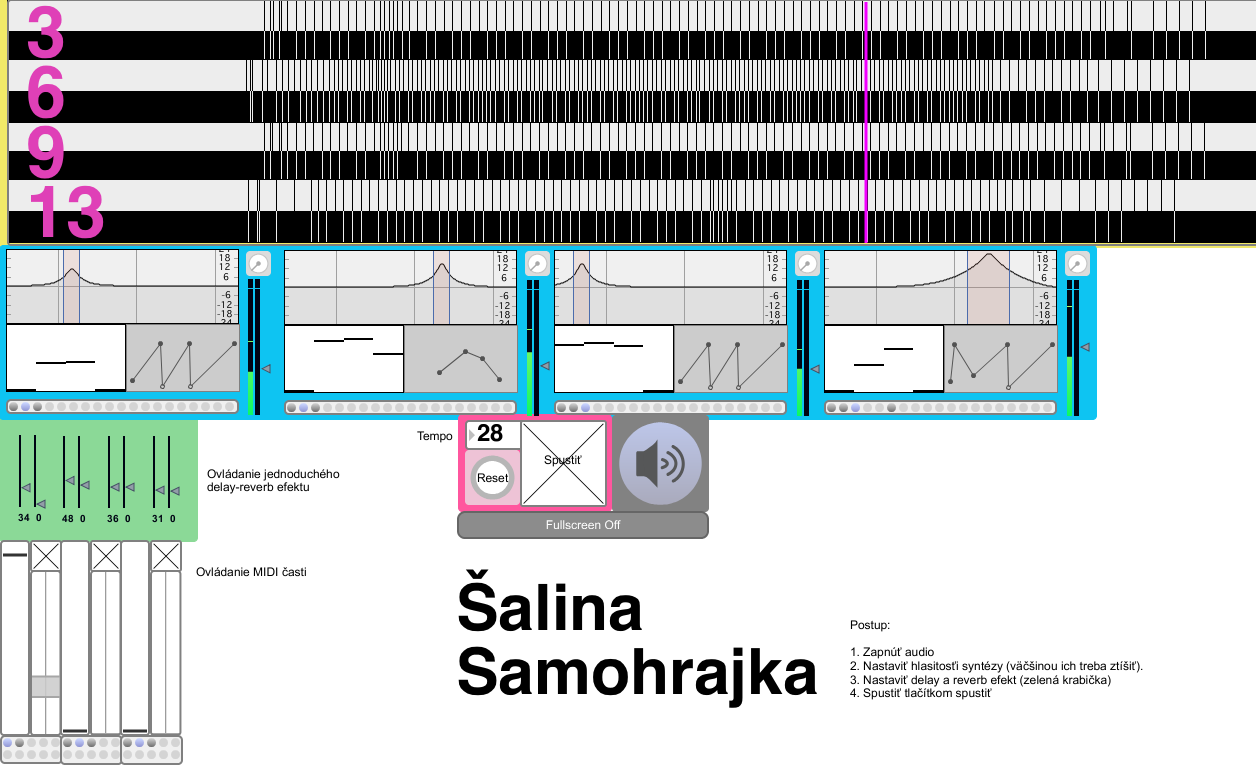
\includegraphics[width=0.9\textwidth]{img/salina}
        \caption{Šalina Samohrajka---timetable sonification Max patch}
        \label{fig:salina}
\end{figure}

Each of the scores (tram lines) represents a binary grid. This means that the timetable had 1440 fields (one for every minute in a day), and a field where no tram arrived was represented by a 0, while the one with a tram arriving was represented by a 1. These scores served as triggers for my percussive synthesizer which was built into the patch. I decided to work with percussive sounds, since my aim was to represent certain kinds of rhythms of the city, or its `breathing'. On the final day of the workshop, I performed (amongst other participants) with this patch. In the performance, I mainly controlled the synthesis and the playback time (the speed of the day) to create various situations and perceptual differences of a time in the city. 

The whole project was a rather interesting experience, but unfortunately I was not able to motivate everyone to do solid work. Many of the people had a natural fear of computers and did not really understand the concepts, which was problematic. But for the ideologically sound ideas (such as the one of Lucie), I now know that it was worth doing.

\begin{figure}  
  \centering
    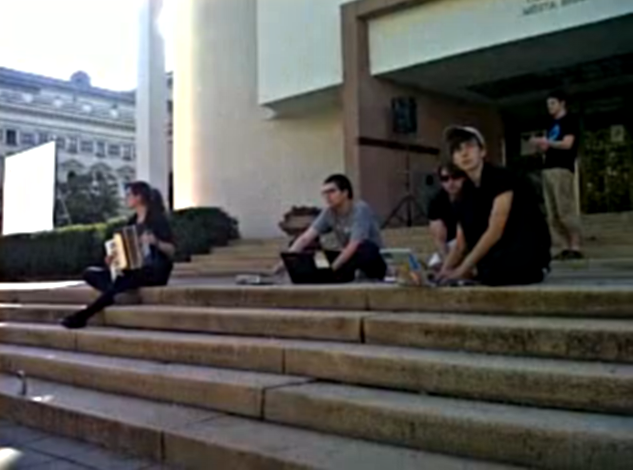
\includegraphics[width=0.9\textwidth]{img/workshop}
        \caption{Street sonification project in front of House of Arts in Brno}
        \label{fig:workshop}
\end{figure}

%%%%%%%%%%%%%%%%%%%%%%%%%%%%%%%%%%%%%%%%%%%%%
%%%%%%%%%%%%%%%%%%%%%%%%%%%%%%%%%%%%%%%%%%%%%

\chapter{Other works} 

\section{Binmatu} Binmatu is an audio-visual drone project that I have been working on and performing with during the last two years.

\subsection{Introduction}

I have never been a very extensive listener of drone music and I could hardly relate to most of the works that I have heard. The idea of extremely slow movements did not please me aesthetically or technically. At the time, I preferred wild improvisations with a high pace of change and an especially high variety of sonic content packed into short compositions.

My horizons were broadened when I heard the works of Phill Niblock and La Monte Young. I realized that drone music needs its own time to be perceived properly. One could say it needs to induce some kind of a trance state, where the listener becomes hypnotized by the simplicity of the composition and the sound. At that point, the subtle changes start to make sense and the whole world of microscopic compositions and performances appears in front of the listener. Our ears (and brain) finally start to focus in on the details, which as under a magnifying glass, have the liberty to become big movements, filled with spine-chilling realizations.

In particular, I was extremely impressed by Phill Niblock's 22 minute long work, \emph{A Trombone Piece}, scored for trombone and tape machine. This piece works as a looper. There are possibly just 2 or 3 notes played (within an interval of a second) during the whole work, yet it creates an astoundingly heavy and dense atmosphere. Nothing really happens in the piece except for the obvious short breaks of the player's breath inhaling before the next upcoming blow. Sonologists may hear comb filtering occurring on overlaying trombone signals, as well as frequency beating (difference tones). Our perception, missing the regular level of stimulation, starts to work differently and becomes more sensitive to the slight details. My own listening changes over the whole duration of the piece, from the regular alert position of a listener to a more meditative and contemplative state of mind. 

\subsection{Starting point}

My own work started during my own musical hibernation. I was at that time doing a residency at OKNO medialab in Brussels, dealing with my project---designing an open-source modular gardening system. Most of the day I was surrounded by the soldering iron and electronic components, or working on some code. I was not communicating with many people during the day and my only companion was a computer (and social contacts accessible through it). It was a strange mental state, where I experienced many hours of silence and loneliness. I feel it is important to describe these conditions, because I believe they are very much reflected in the resulting work. 

I started composing one night. For me as a sonologist, composing often means writing code. To elaborate, after four years at the Institute of Sonology, I sometimes see myself as composer who has exchanged the standard five line staff with (five) lines of code---writing algorithms is writing music to me. And that is what I was doing, writing line after line of code. It started very simply as a few sine waves in specific relationships to each other, slowly coming and going into the space. Bending their frequencies momentarily with almost inaudible results, yet creating something special over the long term. I was immediately charmed by two facts---the simplicity of the composition and the efficiency of such work. I started noticing subtle changes in my state of mind---it was so delicate at first, but after letting my piece play for longer periods of time (10-20 minutes), I was falling into a trance state where the sound would escape the boundaries of its physical body. This experience was at once very frightening, but also very rewarding. I suddenly felt very powerful, and in some way \emph{I was holding sound in my hands}. 

\subsection{Binmatu}

After some time, I ended up with 4 core works. The pieces all used basic sets of oscillators which were modulated by other sets of slower oscillators. All frequencies were picked empirically---\emph{by ear}, based on their sonic impact. I already knew the theory of \emph{binaural beats} and similar psychoacoustic effects, yet I decided to not use those techniques consciously. Rather, I worked more in an empiric fashion of testing and being the test subject.

In the first performances of this project, I experimented with adding my (heavily processed) vocal to the works, but it turned out as a dead end. My views on the whole concept of this particular performance have changed and crystalized into a cleaner, minimalistic perspective. My vocal seemed redundant at this point, and I decided for a more cold, digital, and unstoppable feeling. Singing seemed too weak and somehow pointless against the heavy mass of frequencies. 

At this point, I started to experiment with the strategy of infinite pieces. Something which could be easily faded in and out at any point of its existence and reach the same desired experience. I was looking for a perpetual self-controlling drone, complex enough in its innards to maintain a certain degree of non-repetitiveness (if possible in such a genre). This idea is also present in my other works related to Binmatu, which I mention in more detail later. 

I also started to orient this project to have more of a visual accompaniment, since I have little experience in that field. During my listening sessions, I programmed 4 visual compositions for each piece. The visuals were purposefully not directly connected to music, but were strongly connected in a conceptual sense. They represent the very subtle changes in the music and one needs to experience them for a longer period of time to fully appreciate their potential. This effect is partly achieved by creating \emph{moiré} from huge quantities of primitive shapes and lines. The final visual experience itself is then, in contrast to simplicity of its' essential building blocks, quite complex. This particular effect might be found analogous to sound wave interactions, e.g.\ the beating created by the interaction of two sine waves with close frequencies. Simple lines, when placed together close enough and reduced in the digital domain to pixels, create an effect of pulsating waves and circles due to aliasing, interacting frequencies create a characteristic pulsation of a third frequency born out of the collision of two waves. As it is in the musical component, changes in the video are very slow. Some transitions even take the duration of the whole piece to be noticeable.

\begin{figure}  
  \centering
    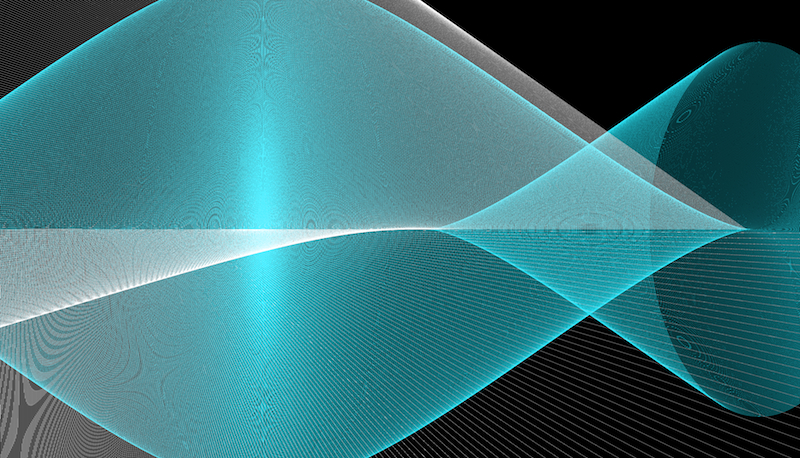
\includegraphics[width=0.9\textwidth]{img/binmatu}
        \caption{One of the Binmatu visuals}
        \label{fig:binmatu}
\end{figure}

From a technical point of view, I am mainly using trigonometric functions for their rhythmic and organic qualities. These are fed with variables which are increasing over the period of the whole piece, and that results in a certain form of repetitive behavior when fed to e.g.\ sine function and linear narrative when used as direct controls of the attributes. The use of color is quite minimalist, as there are rarely more than 2 or 3 colors present at any given time.

After a few performances in Belgium, Czech Republic, Poland, and Slovakia, I was asked to create a new set for performing at the NEXT festival in Slovakia. I composed 9 new works and 9 new visuals in a similar manner to the previous ones. However, this time there appeared to be a slight shift towards other psychoacoustic effects- from binaural beats (as in the first works) towards the Haas effect and other spatial illusions.

One composition in particular is based around time-delayed pulses, where the length of the delay is gradually shifted over time by small steps. I achieved this by setting up two separate pulses (one in each channel), with slight differences in frequency. I calculated the difference in a way that the pulses come to temporary synchronization every 4 minutes (which is the consistent length of my works in this project). The use of pulses brings about another spatial effect- the impulse response of a space. The frequency of the pulses (142 milliseconds) gives sufficient time for revealing the natural resonances and reverberations of any given space. One can also perceive a compressor-like behavior of the ear, which brings (in audio engineering slang, `pumps') more delicate sounds more to the front between each pulse.

\subsection{Selected performances and installations} In this section, I would like to describe and evaluate some of the Binmatu performances and installations. From performances, I have selected the two most recent ones, which are quite different from each other, and that should provide sufficient ground for comparisons. 

The first was a performance in Studio Loos in The Hague during one of the \emph{Ephémère} evenings organized by Marie Guilleray. This event consisted of a stylistic array of performances- from experimental amateur vocal performances of graphic scores (Genetic choir \& Tanja Smit) to the pop songs of Kathrin Grenzdörffer and her project \emph{Glanzkoffer}. Binmatu was scheduled to perform last, which was (from my experiences), a good decision. Unfortunately, by the time of my performance, a large part of the audience had left due to the late hour. Since Studio Loos offers a quadraphonic speaker setup, I decided to use it for my work by mapping the front channels to rear in reverse. During my soundcheck I prepared the speakers in a more traditional symmetrical fashion, but over the course of the night I noticed that the listeners had chosen rather untraditional listening positions in the space, so I improvised and modified the directions of the rear speakers to cover the sides of the small room rather than the center (which was already covered by the front speakers). I was expecting a lot of acoustic interactions such as comb filtering, reverb, and other acoustician's nightmares. Not being an acoustician, I personally enjoyed these effects very much and they became an inspiration for further works and installations.

As expected, the sound was behaving strangely and quickly conquered the whole room. Judging from the perspective of a performer (who is partly out of the system), the transients were completely lost in the reflections and the reverb. The presence of the low frequencies was also slightly lower, but as I said, I was happy with all the imperfections and acoustic errors of the space, because they served my purposes, as they enhanced my work.

The second event I would like to mention, contrasting to the small studio performance, was the \emph{Sonology Discussion Concert} presented in the Arnold Schoenbergzaal of The Royal Conservatory in The Hague. Arnold Schoenbergzall is a spacious concert hall designed for larger events of various genres of music. In all of my years at the Sonology department, it has been the home to most of the Sonology concerts. It was a special moment for me to finally present my work in such a place and I treated it with adequate dignity.

\begin{figure}  
  \centering
    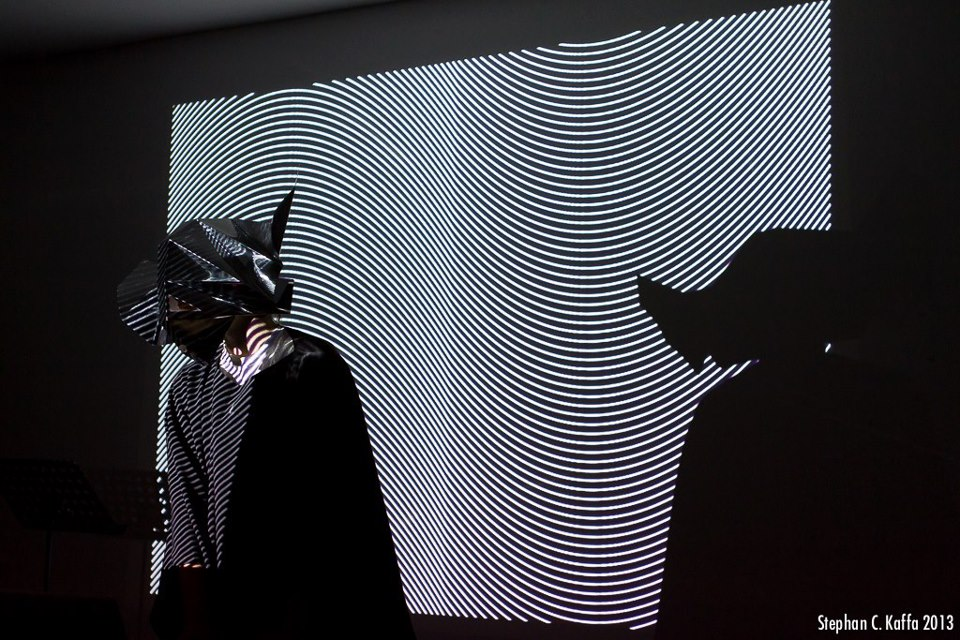
\includegraphics[width=0.9\textwidth]{img/binmatu_perfo}
        \caption{Binmatu performance in Studio Loos}
        \label{fig:binmatu_perfo}
\end{figure}

I have, once again, benefited from a quadraphonic speaker setup, and this time the order the of rear speakers was not reversed. It was quite successful in its realization. There were some minor disturbances with distortion in the speakers and/or mixing console at a few points, but in the end I was satisfied with the results. The hall provided a sufficient ground for the grandiosity of certain pieces, and the previously described `impulse' piece had an enormous impact because of the natural reverberation, which did not smother the transients, yet allowed the blossoming of the impulse responses.

\subsection{Conclusion}

Binmatu will be an ongoing project. Over the course of a year and a half, it has progressed from the uncertain coasts of a self-searching vocal performance to a clean and direct \emph{digitalism}. I still see myself as having a lack of expertise in the performative aspect of this music. I feel that I need to research more artwork that deals with the combination of music and spiritual experiences; ways of reaching deep into human mind (further than simple emotions) through the medium of sound. 

After one of the Binmatu performances, a composer studying classical composition in Slovakia had a very strange experience. He told me that he had ``been places and remembered things which he believed were long forgotten''. I view this as a beautiful compliment, especially because at that point I knew I was not alone in perceiving the psyche-delic (I choose to divide this word to embrace its original meaning) energy stored within these simple sounds. The other compliment that I want to relate was from a girl who said that she was not able to focus on any other music after my performance. My music had worked some kind of special spell which simply did not let her concentrate during the rest of festival. I found this quite beautiful, and I was astonished that my pieces could reach such a level of impact. How far can I possibly reach?

For the future, I see myself starting to work on Binmatu installations as well. It will be an effort to transform my performance into infinite streams of sound and visuals, embracing the site-specificity---using the acoustic properties of space, illusion, and utilizing resonating objects as speakers through the use of tactile transducers.

%%%%%%%%%%%%%%%%%%%%%%%%%%%%%%%%%%%%%%%%%%%%%

\section{Phasolume} Phasolume is an audio-visual installation that I co-authored in collaboration with Agnes Szelag.

\subsection{Introduction} 

During the scholastic year of 2011 / 2012, I was an Erasmus exchange student at the Academy of Music in Kraków. This visit resulted in a few different collaborations. One of my main collaborators was Agnes Szelag, who was on a Fulbright residency at the Academy at the same time.  Agnes is a Polish-American sound artist, performer, composer, and educator. She has performed and presented her work in festivals around the U.S.A. and Europe. She has also authored various audio-visual installations in galleries, museums, and site-specific locations. She received her Master’s Degree in Electronic Music from Mills College in Oakland, California \cite{szelag}.

At the beginning of the year, Szelag started a group called the \emph{Kraków Active Ensemble}, which connected various musicians from the conservatory into a unifying experience of free improvisation and graphic scores. For my part in the group, I mostly used my own software that I had programmed in Max, which I named \emph{JONO}. The ensemble performed at various galleries, electroacoustic events, and open jam sessions.

In the beginning of 2012, Agnes and I decided to collaborate on a sound-based installation. We had both created work in this field before, but our projects and experiences were very different, so it would be interesting to see how things would come together.  We decided that my main role would be in dealing with the technical elements, and her role would be in working with the aesthetic and overall design concept.

\subsection{Working process} 

The root of our idea was to imitate organic behavior and processes observed in nature using sound and light.  We felt that such methods, when used correctly, could relate to some specific parts of our own aesthetic appreciations. Initially, we wanted to permanently place our installation in an abandoned building, but after some research and brainstorming, we changed the plan to create and present the installation directly in my apartment. I had an extra, unfurnished room and it became an ideal environment for working and presenting.  It doesn't often seem to be the case that one has the opportunity to work on a site-based installation without time or space constraints.

By the end of March, we had slowly started to shape a concrete idea and form the specifics of the project. We decided to focus on fireflies (\emph{Lampyris noctiluca}) and their rhythmic and synchronous behavior. We did not set out to make an exact simulation, but rather to recreate an atmosphere of fireflies.  For this purpose, we developed little electronic insects - robots, built from LEDs and vibration motors. The vibration motors were recycled from broken cellphones our friends donated to us.

The main concept became to insert these 10 little robots into various glass jars in a way that they hit the glass with their `bodies' when turned on. This resulted in a very cricket-like sound, since the vibration motors behave like the wings of an insect, especially when turned on in short (one or two second) bursts. This triggered our inspiration and we started to create various sequences with the computer and an Arduino board. Using a sequencing patch I made specifically for this purpose, we were able to work with these robots as with any other MIDI instrument.

\begin{figure}  
  \centering
    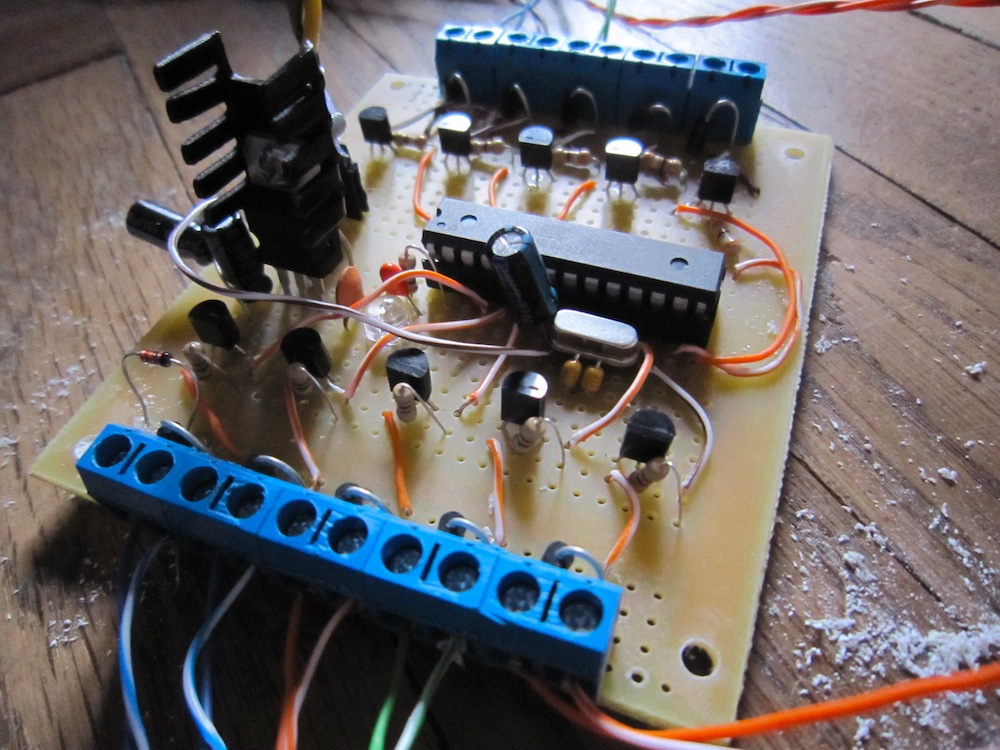
\includegraphics[width=0.9\textwidth]{img/phasolume}
        \caption{Custom designed circuit for Phasolume}
        \label{fig:phasolume}
\end{figure}

An important detail to note was that in the end, the whole system was running without a traditional computer, but instead from a circuit that I designed specifically for this process (see~\ref{fig:phasolume}). This made it possible for the core of the installation to be very small, transportable, and easy to operate.

\subsection{Concept and execution}

After the more technical part of the installation was finished, we started to focus on the sequencing and general aesthetics of the installation.  We abandoned our initial idea of using a pre-programmed (or pre-composed) sequence and started to think more about creating a generative algorithm for the system.

The first algorithmic idea was to create a set of metronomes controlling the rhythms of robots in a fashion similar to Ligeti’s \emph{Poème symphonique}. In this scenario, there would be one metronome per robot with a slightly higher (in linear increments) tempo than the previous, e.g.\ there would be one with a tempo of 60 BPM, the next with 64, the next with 68, and so on. We wanted to create a situation in which the insects would start in sync with each other, then slowly disperse into variations, and eventually return to a sync. After I did some calculations, I concluded that it would be impossible to keep a slow sync start and realize a reasonable length for the whole cycle (from sync to sync). According to my calculations, the cycle length would range from tens of hours to hundreds of days. The participant’s perception of synchronization was at the core of our concept, so we decided to create artificial resets---resynchronizations---so that a participant could experience a few during their visit (generally 5-10 minutes of active observation per person). During resynchronization, a new set of tempos would be picked from the database and the whole sequence would start again.

The whole installation was set up (as mentioned) in my apartment with the power core of the system installed in the ceiling instead of a lamp. I replaced the lamp with an electrical socket, so in the end it was possible to turn on the whole installation just by flipping a standard light switch.

\subsection{Exhibition}

After a successful exhibition at my apartment (and only slight problems with the police), we were invited to present the installation at Krakers. Krakers is a yearly event happening in Kraków which is dedicated to presenting small art collectives in mostly home galleries. I set up the installation in another apartment and all together it was visited by more than 250 people. During the second installation, many people stayed with it for longer periods of time, simply enjoying the patterns emerging from the desynchronicity of the metronomic behavior.

\subsection{Conclusion}

I really enjoyed this method of working, as well as the collaboration with an artist who came from such a different background and context. I believe it resulted in a fruitful combination of technical and aesthetic worlds and helped me with my own personal attitude towards creating more public works of this kind in the future.

%%%%%%%%%%%%%%%%%%%%%%%%%%%%%%%%%%%%%%%%%%%%%

\section{Site Specific Resonances}

\subsection{Introduction}

\emph{Site Specific Resonances} was my latest project during the period of writing of this thesis. It was a sound installation exhibited in the Vrije Academie Gemak in The Hague.

The project started with my proposal to the gallery for creating a site-specific sound installation. My aim was to research a few topics close to my aesthetics---minimalism, hidden technology, and the reusing/repurposing of materials. In the end, it turned out quite differently---instead of creating a permanent installation, I built a special environment to perform with. 

I see this project as something of a continuation of my Binmatu project, where I am focusing on drones and subtle psychoacoustic effects hidden in the compositions.

For this installation, I decided to work with the resonant frequencies of the space. By measuring the room acoustics with a measurement microphone and an impulse response, I extracted the most resonant frequencies and began composing.

\subsection{Technical aspects}

It is important to mention that I decided (as part of the minimalist aesthetics) not to use traditional speakers. I see them as somehow distracting elements. In addition, the method I used instead---tactile transducers---worked much better visually and sonically.

\begin{figure}  
  \centering
                \tikzstyle{block} = [rectangle, draw, 
                    text width=7em, text centered, minimum height=2.5em, node distance=3cm,
                        %top color=white, % a shading that is white at the top...
                        %bottom color=black!10,
                        rounded corners=2pt] % and something else at the bottom]
                \tikzstyle{line} = [draw, -triangle 90, rounded corners=5pt]


                \begin{tikzpicture}[node distance = 2cm, auto]
                    % Place nodes
                    \node [block] (me) {\textbf{Me} \\ (Performer)};
                        \node [block, below of=me, xshift=-5em, node distance=3.6cm] (raspi) {Raspberry Pi \\ running ChucK};
                        \node [block, below of=me, xshift=5em, node distance=2.5cm] (amp1) {Amplifier 2};
                        \node [block, below of=raspi, node distance=2.8cm] (amp2) {Amplifier 1};
                        \node [block, below of=amp1, node distance=1.8cm] (trans1) {Transducer 2};
                        \node [block, below of=amp1, node distance=1.8cm, xshift=10em] (trans2) {Transducer 3};
                        \node [block, below of=amp2, node distance=1.8cm] (trans3) {Transducer 1};

                    % Draw edges
                    \path [line, dashed] (me) -| node [near end, above, scale=.8, rotate=90, align=center, text centered, text width=3cm] {wireless \\ remote control} (raspi);
                        \path [line] (me) -| node [near end, below, scale=.8, rotate=90] {audio} (amp1);
                        \path [line] (raspi) -- node [above, scale=.8, rotate=90] {audio} (amp2);
                        \path [line] (amp1) -- (trans1);
                        \path [line] (amp1) -| (trans2);
                        \path [line] (amp2) -- (trans3);

                        \begin{scope}[on background layer]
                            \node[fill=lightgray!50,inner sep = 3mm,fit=(trans1),label=below:Metallic Plate 2] {}; 
                                \node[fill=lightgray!50,inner sep = 3mm,fit=(trans2),label=below:Oil barrel] {}; 
                                \node[fill=lightgray!50,inner sep = 3mm,fit=(trans3),label=below:Metallic Plate 1] {};
                        \end{scope}

        \end{tikzpicture}
        \caption{System of \emph{Site Specific Resonances} installation}
        \label{fig:sitespec}
\end{figure}


Tactile transducers are basically moving magnetic coils (like the ones found in any speaker), but without the speaker cone. They can be attached to any object which has a vibrate-able body. Tactile transducers utilize the body of the object as a speaker cone and in result, the object then becomes a speaker. 

This, of course, brings many interesting aspects to the newly-created sound emitter. Primarily, it is inheriting the acoustic imperfections of the object. E.g.\ a metallic plate resonates at certain frequencies and presents a long reverb (such as is found in plate reverb). I have exercised this concept greatly in my project.

First, I acquired various interesting objects which were lying around the workshop of the gallery---two metallic plates and one empty oil barrel. Then I created three different `stages', three different sound emitting objects. Two of those were connected to one amplifier and then to my computer, and one stage was totally separate from the main computer. To achieve this visual separation---no cables running through the space. This was important to me, since I often find cables visually distracting. My goal was the element of surprise, the perception of the object as a truly autonomous sound-emitting unit. To accomplish that, I used a few different technologies that I had on hand. The sounds were generated from a Raspberry Pi microcomputer running the sound programming language Chuck. This audio was then fed to a small amplifier and finally to the object (or rather, to the transducer connected to it). For a better visualization of this concept, I have created figure~\ref{fig:sitespec}.

This solution gave me the opportunity to have total control over what was happening in the room sound-wise, without the need for a jungle of wires and multichannel sound cards. It became especially important when my work in the gallery became more focused on performing with the objects rather than creating a standalone self-sustaining installation.

Visually, the installation looked very minimalist---bare metallic plates emitting sound and one rambling oil can, shaking in a fearful drone. I personally find something very intriguing about simple metallic objects in space, especially when standing on their own; simple and raw in their full glory. They are like simple and understandable statements in a book, yet they offer a few different perspectives.

\subsection{Performances}

I have performed with the tactile transducers a total of 5 times for various groups of people. The first performances were happening during the Hoogtij event which turned out to be quite unfortunate. The nature of the Hoogtij crowds and the delicate sound installation simply did not come together as a good match, as I had to ask people to be quiet many times to make my work audible. Luckily, the last three performances (after the first two unsuccessful performances) went quite well, and one even turned out to get a very positive review on a local art blog \cite{jegen}.

\subsection{Conclusion and future}

The clear message coming from the presentation of these works is to prepare the audience as much as possible for what is being presented. Otherwise, the subtle details which I base my work on go unnoticed and unexperienced, and in the end become worthless.

This project gave me a lot of inspiration for future works, and I have already been asked by the director of the gallery to create something new for their space.

I have actually quite enjoyed the concept of creating an installation which serves as a system for performance, and performing on non-traditional setups gives a beautiful atmosphere to the work and creates a very different listening situation from the one we all know. 

\begin{figure}  
  \centering
    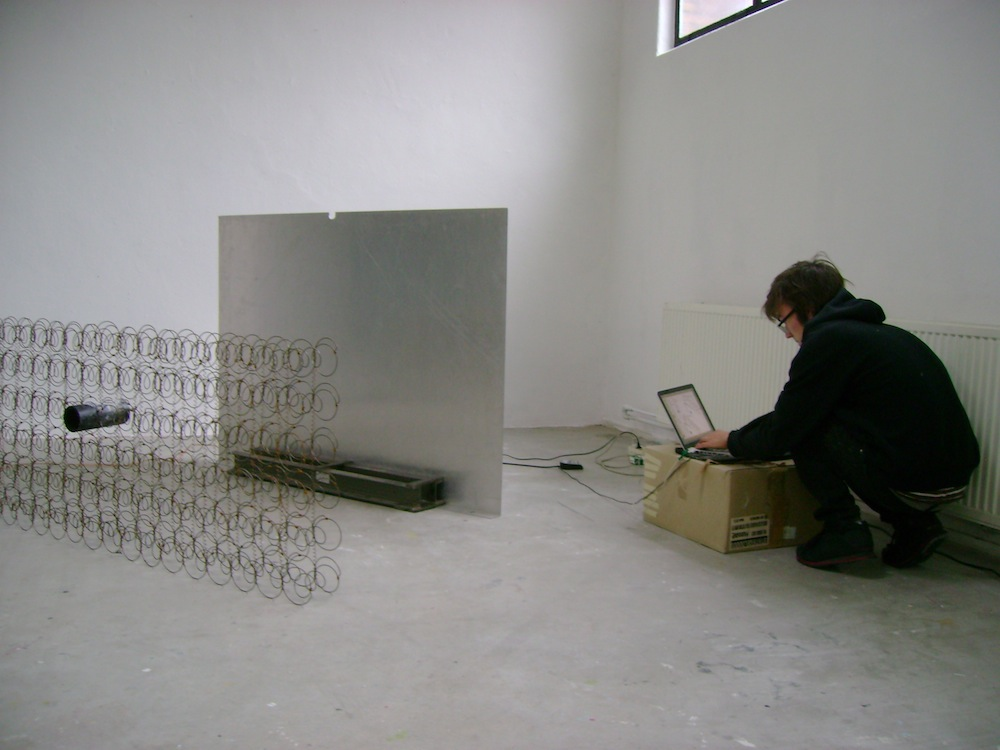
\includegraphics[width=1\textwidth]{img/sitespec}
        \caption{Performance of \emph{Site Specific Resonances}}
        \label{fig:sitespec}
\end{figure}

\chapter{Conclusion}
In conclusion, I believe that I have managed to give you a glimpse of my views on sonification and its current status in the artistic, as well as the scientific universe. I provided a few clear examples of what the artistic sonification is and might be. I am hoping to see more and more collaborations of arts and sciences, which might help us to understand difficult concepts; but I also hope to see more uses of purely artistic sonification, which I have fallen in love with over my last few years. I want to hear the inner workings of the machines which surround us on daily basis. To hear the invisible data streams transmitting infinite amounts of data through our tissues. To hear an to listen, to learn and to improve, to experience non-auditory aspects of our world through eardrum oscillations, and the wonderful apparatus hidden behind them.

My future plans are still very misty, but I feel like I do not want to sink completely into the technology. By itself it is delightful, but not powerful enough. It is the combination of my artworks, which is supposed to bring them to life, bring the life to the electrons in their tangled conductive veins. It is not an easy task to stay in the mindset of an artist and an engineer at the same time. But I will try, jump through, and hoping not fall far from concepts just for the superficial beauty of circuit boards and code. I want to remain an artist in a first place, and I hope the descriptions of my latest projects have not proved me differently. 

The shift over last 4 years has turned me from the extremely fast and dense compositions to the psychedelic minimalism, yet I do not think of it as of the evolution. I would say it is my inner need for change, change of the environments, approaches, the experiment. There is no better stage, just different. It is the same driving force, which led me from repairing old bicycles to picking locks, through hacking wireless networks to designing hardware electronics. I do not want to stay at one place and recycle myself, I need to explore and dive into new realms. That is the only way for me to reach new levels of understanding world and thus creating more and precise, powerful art.

\onehalfspacing

\bibliographystyle{apacite} 
\bibliography{general}

\appendix
\chapter{List of selected performances, exhibitions, workshops and lectures}
\singlespacing

\textbf{2011}
\begin{itemize}
\item Participating in workshop of Seijiro Murayama and performing in A4, Bratislava
\item Exhibiting finnish version of interactive poem Basen at Live Herring 2011 festival in Finland
\item Solo exhibition - interactive installation about 4 modes of listening at Royal Conservatory, Den Haag
\item Leading 4-day workshop on untraditional ways of city sonification, Brno, Czech Republic
\item Leading workshop on Pure Data, audio programming and Processing and performing on Intermedia festival in Banská Bystrica, Slovakia
\item Performing on AudioArt festival, Cracow, Poland. Exhibiting live sound installation Sonodump, Krakow, Poland
\item Performing on NEXT festival, Bratislava Slovakia
\end{itemize}
\vspace{1cm}

\textbf{2012}
\begin{itemize}
\item Performing with Krakow Active Ensamble in Alchemia, Krakow, Poland
\item BINMATU performance on Progressbar birthday party, Bratislava, Slovakia
\item Artistic residency at OKNO, Brussels, Belgium
\item Performing at OEN, Krakow, Poland
\item Artistic presentation and performance at Multiplace festival, Brno, Czech Republic
\item BINMATU performance in Academy of Music, Krakow, Poland
\item OSMOGAS exhibition at TIK festival, Brussels, Belgium
\item OSMOGAS exhibition at Open House festival, Brussels, Belgium
\item BINMATU performance at TIK festival, Brussels, Belgium
\item BINMATU performance at Queerowy maj, Krakow, Poland
\item Performing with Krakow Active Ensamble in Alchemia, Krakow, Poland
\item Performing with Krakow Active Ensamble at Index errorum dzieciorum installation opening, Krakow, Poland
\item Phasolume installation with Agnes Szelag, Krakow, Poland
\item BINMATU performance at Dietla 449, Krakow, Poland
\item BINMATU performance at Slovak Radio, Bratislava, Slovakia
\item Leading workshop on digital audio, Pure Data and programming at Young composers festival, Bratislava, Slovakia
\item BINMATU performance at NK, Bratislava, Slovakia
\item BINMATU performance at Day of Sound, Bunkier Sztuki, Krakow, Poland
\item Performing at Haguestock, Den Haag, Netherlands
\item Performing with Luke Deane and Eugene Kim, Den Haag, Netherlands
\item BINMATU performance at NEXT festival, Slovakia
\end{itemize}
\vspace{1cm}

\textbf{2013}
\begin{itemize}
\item BINMATU performance at Ephemere, Den Haag, Netherlands
\item Performing at Art's Birthday, Brussels, Belgium
\item BINMATU performance at Institute of Sonology, Den Haag, Netherlands
\item Performing at Haguestock, Den Haag, Netherlands
\item Performing at LOM label showcase, Bratislava, Slovakia
\item Performing at Kraak festival, Aalst, Belgium
\item Performing with Bolka, Den Haag, Netherlands
\item Performing in Gemak gallery, Den Haag, Netherlands
\end{itemize}

\chapter{List of links to my projects}
\singlespacing
\begin{itemize}
\item My personal website \\ \url{http://mrkva.ovecka.be}
\item Binmatu website \\ \url{http://binmatu.net}
\item LOM (label I have founded) website \\ \url{http://zvukolom.org}
\item Phasolume project \\ \url{http://mrkva.ovecka.be/index.php?/interactive/phasolume-11/}
\item AudioArt ("Sonodump") performance \\ \url {https://vimeo.com/33858336}
\end{itemize}


\end{document} 
